
\newsavebox{\GradeAssignmentCA}
\begin{lrbox}{\GradeAssignmentCA}
\begin{lstlisting}[language=C++,style=smaller]
int GradeAssignment(FILE *in) {
  int scores[10]; char buffer[16];
  for (int i = 0; i < 10; ++i) {
    gets(buffer);
    scores[i] =
        GradeAnswer(buffer, i);
  }
  Process(scores);
}
\end{lstlisting}
\end{lrbox}

\newsavebox{\GradeAssignmentAsmA}
\begin{lrbox}{\GradeAssignmentAsmA}
\begin{lstlisting}[language=myasm,style=smaller,morekeywords=incl]
GradeAssignment:
  pushq   %rbp
  pushq   %rbx
  xorl    %ebx, %ebx
  subq    $72, %rsp
  leaq    8(%rsp), %rbp
for_loop:
  movq    %rbp, %rdi
  call    gets
  movl    %ebx, %esi
  movq    %rbp, %rdi
  call    GradeAnswer
  leaq    24(%rsp), %rdi
  movl    %eax, (%rdi,%rbx,4)
  incq    %rbx
  cmpq    $10, %rbx
  jne     for_loop
  call    Process
  ...
\end{lstlisting}
\end{lrbox}

\begin{frame}[fragile,label=simpleOverStackLayout1]{exercise: stack layout}
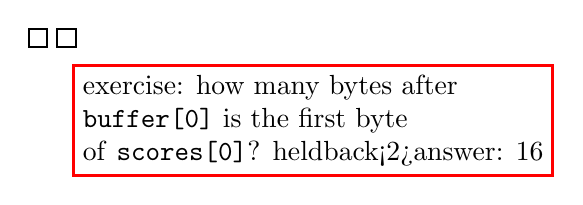
\begin{tikzpicture}
\node[draw,thick] (c code) {%
\usebox{\GradeAssignmentCA}
};
\node[draw, thick,anchor=north east] (asm code) at ([xshift=-1mm]c code.north west) {%
\usebox{\GradeAssignmentAsmA}
};
\node[draw=red,very thick,anchor=north west,align=left] at ([xshift=2mm,yshift=-2mm]c code.south west) {
exercise: how many bytes after \\
\texttt{buffer[0]} is the first byte \\
of \texttt{scores[0]}?
\iftoggle{heldback}{}{\only<2>{answer: 16}}
};
\end{tikzpicture}
\end{frame}

\begin{frame}[fragile,label=simpleOverStackLayout2]{exercise: overflow?}
\begin{tikzpicture}
\node[draw,thick] (c code) {
\usebox{\GradeAssignmentCA}
};
\node[draw, thick,anchor=north east] (asm code) at ([xshift=-1mm]c code.north west) {
\usebox{\GradeAssignmentAsmA}
};
\node[draw=red,very thick,anchor=north west,align=left] at ([xshift=2mm,yshift=-2mm]c code.south west) {
exercise: if input into buffer is \\
50 copies of the character \texttt{'1'} \\
what is value of \texttt{scores[0]}?
\iftoggle{heldback}{}{\only<2>{\\answer: 0x31313131}}
};
\end{tikzpicture}
\end{frame}
